\documentclass[10pt,landscape,a4paper]{article}
\usepackage[utf8]{inputenc}
\usepackage[UKenglish]{babel}
\usepackage{tikz}
\usetikzlibrary{shapes,positioning,arrows,fit,calc,graphs,graphs.standard}
\usepackage[nosf]{kpfonts}
\usepackage[t1]{sourcesanspro}
%\usepackage[lf]{MyriadPro}
%\usepackage[lf,minionint]{MinionPro}
\usepackage{multicol}
\usepackage{wrapfig}
\usepackage[top=0mm,bottom=4mm,left=2mm,right=1mm]{geometry}
\usepackage[framemethod=tikz]{mdframed}
\usepackage{microtype}
\usepackage{mathtools} % loads amsmath, for math environments etc
\usepackage{setspace}
\usepackage{tikz}
\usetikzlibrary{trees}
\usepackage{enumitem}
\usepackage{kpfonts,amssymb,empheq,fancybox}

\usepackage{graphicx}
\usepackage{tikz}
\usetikzlibrary{arrows,shapes,positioning}

\usepackage{pgfplots}
\usepackage{venndiagram}

\let\bar\overline
\let\displaystyle\textstyle

\definecolor{myblue}{cmyk}{1,.72,0,.38}

\def\firstcircle{(0,0) circle (1.5cm)}
\def\secondcircle{(0:2cm) circle (1.5cm)}

\colorlet{circle edge}{myblue}
\colorlet{circle area}{myblue!5}

\tikzset{filled/.style={fill=circle area, draw=circle edge, thick},
    outline/.style={draw=circle edge, thick}}

\pgfdeclarelayer{background}
\pgfsetlayers{background,main}

\everymath\expandafter{\the\everymath \color{myblue}}
\everydisplay\expandafter{\the\everydisplay \color{myblue}}

\renewcommand{\baselinestretch}{.8}
\pagestyle{empty}

\global\mdfdefinestyle{header}{%
linecolor=gray,linewidth=1pt,%
leftmargin=6mm,rightmargin=6mm,skipbelow=1mm,skipabove=1mm,
}

\newcommand{\ffbox}[1]{%
	{% open a group for a local setting
		\setlength{\fboxsep}{-2\fboxrule}% the rule will be inside the box boundary
		\fbox{\hspace{1.2pt}\strut#1\hspace{1.2pt}}% print the box, with some padding at the left and right
	}% close the group
}

\newcommand{\header}{
\begin{mdframed}[style=header]
\scriptsize

\textbf{Probability with Martingales booklet by~Alain~Chenier,~page~\thepage~of~2,  \today{} }
\end{mdframed}
}

\makeatletter
\renewcommand{\section}{\@startsection{section}{1}{0mm}%
                                {.1ex}%
                                {.1ex}%x
                                {\color{blue}\sffamily\small\bfseries}}
\renewcommand{\subsection}{\@startsection{subsection}{1}{0mm}%
                                {.1ex}%
                                {.1ex}%x
                                {\sffamily\bfseries}}

\def\textSq#1{%
	\begingroup% make boxes and lengths local
	\setlength{\fboxsep}{0.001pt}% SET ANY DESIRED PADDING HERE
	\setbox1=\hbox{#1}% save the contents
	\setlength{\@tempdima}{\maxof{\wd1}{\ht1+\dp1}}% size of the box
	\setlength{\@tempdimb}{(\@tempdima-\ht1+\dp1)/2}% vertical raise
	\raise-\@tempdimb\hbox{\fbox{\vbox to \@tempdima{%
				\vfil\hbox to \@tempdima{\hfil\copy1\hfil}\vfil}}}%
	\endgroup%
}
\def\Sq#1{\textSq{\ensuremath{#1}}}%

\def\multi@column@out{%
   \ifnum\outputpenalty <-\@M
   \speci@ls \else
   \ifvoid\colbreak@box\else
     \mult@info\@ne{Re-adding forced
               break(s) for splitting}%
     \setbox\@cclv\vbox{%
        \unvbox\colbreak@box
        \penalty-\@Mv\unvbox\@cclv}%
   \fi
   \splittopskip\topskip
   \splitmaxdepth\maxdepth
   \dimen@\@colroom
   \divide\skip\footins\col@number
   \ifvoid\footins \else
      \leave@mult@footins
   \fi
   \let\ifshr@kingsaved\ifshr@king
   \ifvbox \@kludgeins
     \advance \dimen@ -\ht\@kludgeins
     \ifdim \wd\@kludgeins>\z@
        \shr@nkingtrue
     \fi
   \fi
   \process@cols\mult@gfirstbox{%
%%%%% START CHANGE
\ifnum\count@=\numexpr\mult@rightbox+2\relax
          \setbox\count@\vsplit\@cclv to \dimexpr \dimen@-1cm\relax
\setbox\count@\vbox to \dimen@{\vbox to 1cm{\header}\unvbox\count@\vss}%
\else
      \setbox\count@\vsplit\@cclv to \dimen@
\fi
%%%%% END CHANGE
            \set@keptmarks
            \setbox\count@
                 \vbox to\dimen@
                  {\unvbox\count@
                   \remove@discardable@items
                   \ifshr@nking\vfill\fi}%
           }%
   \setbox\mult@rightbox
       \vsplit\@cclv to\dimen@
   \set@keptmarks
   \setbox\mult@rightbox\vbox to\dimen@
          {\unvbox\mult@rightbox
           \remove@discardable@items
           \ifshr@nking\vfill\fi}%
   \let\ifshr@king\ifshr@kingsaved
   \ifvoid\@cclv \else
       \unvbox\@cclv
       \ifnum\outputpenalty=\@M
       \else
          \penalty\outputpenalty
       \fi
       \ifvoid\footins\else
         \PackageWarning{multicol}%
          {I moved some lines to
           the next page.\MessageBreak
           Footnotes on page
           \thepage\space might be wrong}%
       \fi
       \ifnum \c@tracingmulticols>\thr@@
                    \hrule\allowbreak \fi
   \fi
   \ifx\@empty\kept@firstmark
      \let\firstmark\kept@topmark
      \let\botmark\kept@topmark
   \else
      \let\firstmark\kept@firstmark
      \let\botmark\kept@botmark
   \fi
   \let\topmark\kept@topmark
   \mult@info\tw@
        {Use kept top mark:\MessageBreak
          \meaning\kept@topmark
         \MessageBreak
         Use kept first mark:\MessageBreak
          \meaning\kept@firstmark
        \MessageBreak
         Use kept bot mark:\MessageBreak
          \meaning\kept@botmark
        \MessageBreak
         Produce first mark:\MessageBreak
          \meaning\firstmark
        \MessageBreak
        Produce bot mark:\MessageBreak
          \meaning\botmark
         \@gobbletwo}%
   \setbox\@cclv\vbox{\unvbox\partial@page
                      \page@sofar}%
   \@makecol\@outputpage
     \global\let\kept@topmark\botmark
     \global\let\kept@firstmark\@empty
     \global\let\kept@botmark\@empty
     \mult@info\tw@
        {(Re)Init top mark:\MessageBreak
         \meaning\kept@topmark
         \@gobbletwo}%
   \global\@colroom\@colht
   \global \@mparbottom \z@
   \process@deferreds
   \@whilesw\if@fcolmade\fi{\@outputpage
      \global\@colroom\@colht
      \process@deferreds}%
   \mult@info\@ne
     {Colroom:\MessageBreak
      \the\@colht\space
              after float space removed
              = \the\@colroom \@gobble}%
    \set@mult@vsize \global
  \fi}

\makeatother
\setlength{\parindent}{0pt}
\setlength{\columnseprule}{0.01pt}


\begin{document}
\scriptsize
\begin{multicols*}{3}

\setlength\fboxsep{0.5 pt}
\textbullet Distribution of \boxed{Z_n} obtained from generating $ \Rightarrow f_n(\theta)  =  E(\theta^{Z_n}) = \sum \theta^k \boxed{ P(Z_n=k) }$ \\
\textbullet $ f_{n+1}(\theta) = E  \theta^{Z_{n+1} } = E \left(  \boxed{E\theta^{Z_{n+1}}|Z_n} \right) = \sum \boxed{E  \left( \theta^{Z_{n+1}} | Z_n    \right)}  P(Z_n=k) \leftarrow \boxed{E  \theta^{Z_{n+1}} | Z_n}     $ is the random variable here \\

\begin{spacing}{0.1}
	
\section{Chapter 0}

\begin{mdframed}[style=header]	
$\mathbf{Z+}=[0,1..] \quad \mathbf{N}=[1..] \\
f(\theta)=E(\theta^X) = \sum \theta^k P(X=k) = P(X-0) + \sum_{k=1} \theta^k P(X=k) \\
f'(\theta)=E(\theta^X) = \sum k \theta^{k-1} P(X=k) \leftarrow \text{differentiate wrt } \theta \\
\text{mean} = \mu = f'(1) = \sum_k k P(X=k) \quad f(1) = \sum P(X=k) = 1
$ \\
\end{mdframed}

$ \{X_r^m\} = \text{double series of random variables IID  } \\ 
X_{r+1}^m= \text{the children in r+1 generation} \\
Z_{r+1}^m= X_{1}^m + ... + X_{Z_r}^m = \text{sum of the children in r+1 generation} \\
$

\subsection{my example}

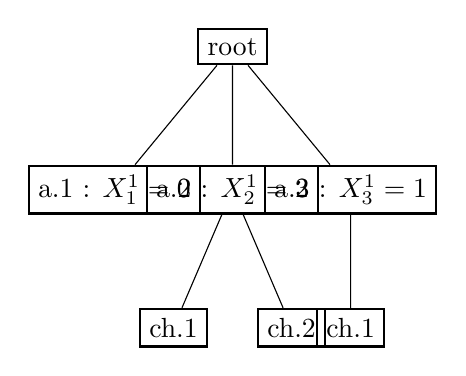
\begin{tikzpicture} 
\begin{scope}
\tikzstyle {every node}=[draw=black,thick,anchor=north] 

\node {root}
child { node {a.1 : $X_1^1=0$}
}		
child { node {a.2 : $X_2^1=2$}
	child { node {ch.1}}
	child { node {ch.2}}
}
child { node {a.3 : $X_3^1=1$}
child { node {ch.1}}
};
\end{scope}

\end{tikzpicture}


\section{Chapter 0}

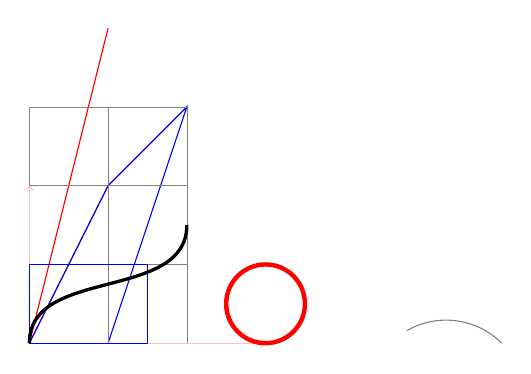
\begin{tikzpicture}
\draw   [red]  (0,0) --(1,2);
\draw  [blue]  (0,0) --(1,2) -- (2,3) -- (1,0);
\draw [red](0,0) --(1,4);
\draw[help lines] (0,0) grid (2,3);
\draw [<->] [pink] (0,2) -- (0,0) -- (3,0);
\draw [blue] (0,0) rectangle (1.5,1);
\draw [red, ultra thick] (3,0.5) circle [radius=0.5];;
\draw [gray] (6,0) arc [radius=1, start angle=45, end angle= 120];
\draw[very thick] (0,0) to [out=90,in=-90] (2,1.5);
\end{tikzpicture}


\section{Chapter 0}

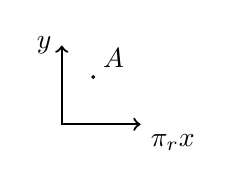
\begin{tikzpicture}

\draw [thick, <->] (0,1) node [left] {$y$} -- (0,0) -- (1,0) node [below right] {$\pi_{r}x$};
\draw (.4,.6) circle [radius=.5pt] node[above right] (.4,.6) {$A$};


\end{tikzpicture}

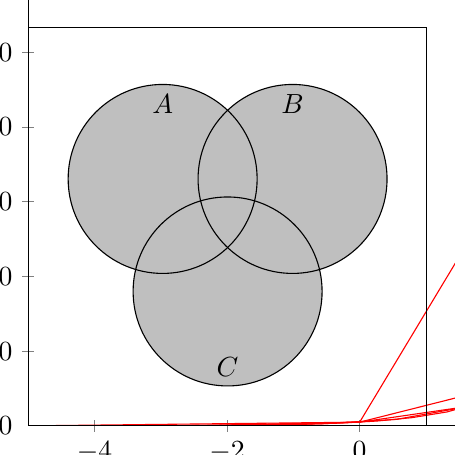
\begin{tikzpicture}
\pgfplotsset{width=10cm,compat=1.9}
\begin{axis}
[
axis lines = left,
xlabel = $x$,
ylabel = {$f(x)$},
]
\addplot[color=red,domain=-5:5,samples=3, color=red,]{exp(x)};
\addlegendentry{$x^2 + 2x + 1$}
\addplot[color=red,domain=-5:5,samples=5, color=red,]{exp(x)};
\addplot[color=red,domain=-5:5,samples=7, color=red,]{exp(x)};
\addplot[color=red,domain=-5:5,samples=10, color=red,]{exp(x)};
\addplot[color=red,domain=-5:5,samples=20, color=red,]{exp(x)};
\end{axis}

\begin{venndiagram3sets}
\fillA \fillB \fillC
\end{venndiagram3sets}



\end{tikzpicture}
%Here ends the furst plot
\hskip 5pt

\begin{equation}
\begin{split}
H_{1mmmmm} & = \{W_{2}(x), W_{1}(x), R_{3}(x), R_{1}(x), W_{2}(y), R_{3}(y), R_{3}(z), R_{2}(x)\} \\
H_{gggg2} & = \{R_{3}(z), R_{3}(y), W_{2}(y), R_{2}(z), W_{1}(x), R_{3}(x), W_{2}(x), R_{1}(x)\} \\
H_{3ggg} & = \{R_{3}(z), W_{2}(x), W_{2}(y), R_{1}(x), R_{3}(x), R_{2}(z), R_{3}(y), W_{1}(x)\} \\
H_{4g} & = \{R_{2}(z), W_{2}(x), W_{2}(y), W_{1}(x), R_{1}(x), R_{3}(x), R_{3}(z), R_{3}(y)\}
\end{split}
\end{equation}


\pgfplotsset{compat=1.6}

\pgfplotsset{soldot/.style={color=blue,only marks,mark=*}} \pgfplotsset{holdot/.style={color=blue,fill=white,only marks,mark=*}}

	
	\begin{tikzpicture}
	\begin{axis}
	\addplot[domain=1.8:2,blue] {x*x};
	\addplot[domain=2:2.2,blue] {x*x+1};
	\draw[dotted] (axis cs:2,0) -- (axis cs:2,5);
	\addplot[holdot] coordinates{(2,4)};
	\addplot[soldot] coordinates{(2,5)};

	\draw[dotted] (axis cs:0,4.5) -- (axis cs:2,4.5);

	\draw[->] (axis cs:1.9, 1.9*1.9+0.1) -- (axis cs:1.95, 1.95*1.95+0.1);
	\draw[<-] (axis cs:2.05, 1+2.05*2.05+0.1) -- (axis cs:2.1, 2.1*2.1+0.1+1);

    \node[anchor=east] (source) at (axis cs:2.1,5){\text\ F(x)};
    \node[anchor=east] (source) at (axis cs:1.95,3.5){\text\ F(x)};

    \node[anchor=north](source) at (axis cs:1.8,4.6){$\omega$};
    \node[anchor=south](source) at (axis cs:2,3.2){$X^{+/-}(\omega)$};

	\end{axis}
	\end{tikzpicture}


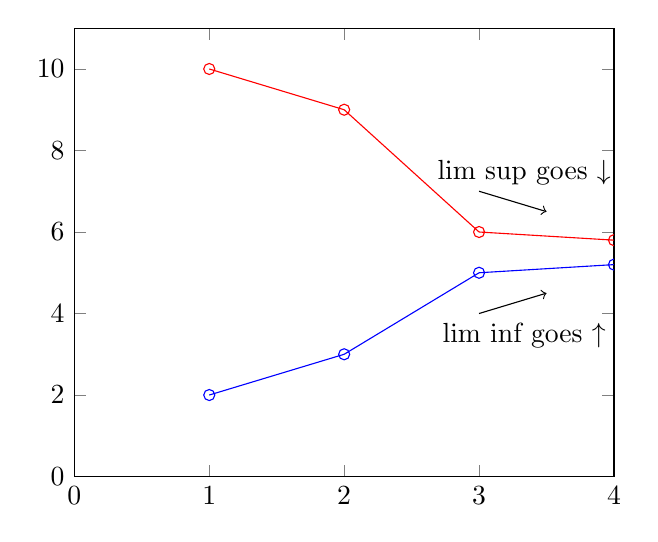
\begin{tikzpicture}
\begin{axis} [  xmin=-0, xmax=4, ymin=0,ymax=11]

	\draw[red] (axis cs:1,10) circle[radius=2pt] -- (axis cs:2,9) circle[radius=2pt] -- (axis cs:3,6) circle[radius=2pt] -- (axis cs:4,5.8) circle[radius=2pt];
	
	\draw[blue] (axis cs:1,2) circle[radius=2pt] -- (axis cs:2,3) circle[radius=2pt] -- (axis cs:3,5) circle[radius=2pt] -- (axis cs:4,5.2) circle[radius=2pt];

    \node[anchor=north] (source) at (axis cs:3.3,8){ \text\ lim sup goes $\downarrow$};
    \node[anchor=north] (source) at (axis cs:3.3,4){\text\ lim inf goes $\uparrow$ };

	\draw[->] (axis cs:3, 4) -- (axis cs:3.5, 4.5);
	\draw[->] (axis cs:3, 7) -- (axis cs:3.5, 6.5);

\end{axis}
\end{tikzpicture}


\end{spacing}
\end{multicols*}
\end{document}